\setlength{\LTpre}{0pt}
\setlength{\LTpost}{0pt}
\small
\renewcommand{\arraystretch}{1.1}
\setlength{\tabcolsep}{3pt}
\begin{longtable}{C{3.4cm}C{3.7cm}C{7.0cm}}
\caption{Ligantes comerciais e de referência selecionados para a triagem, com desenhos do Apêndice B e fontes das estruturas ou dos complexos cristalográficos.}\label{tab:ligantes_comerciais_justificativa}\\
\toprule Ligante & Estrutura bidimensional & Fonte da estrutura ou referência \\
\midrule
\endfirsthead
\multicolumn{3}{c}{\tablename~\thetable\ (continuação)}\\
\toprule Ligante & Estrutura bidimensional & Fonte da estrutura ou referência \\
\midrule
\endhead
\midrule
\multicolumn{3}{r}{Continua na próxima página}\\
\endfoot
\bottomrule
\endlastfoot
ARP-100 & 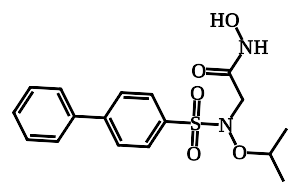
\includegraphics[width=3.2cm,height=0.9cm,keepaspectratio]{image/estruturas_ligantes_integracao/miniaturas/com_ARP_100.png} & Estrutura química consultada no PubChem \parencite{pubchem2023} \\
Ácido ascórbico & 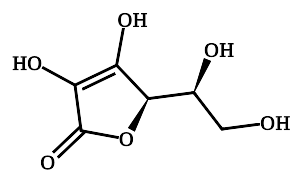
\includegraphics[width=3.2cm,height=0.9cm,keepaspectratio]{image/estruturas_ligantes_integracao/miniaturas/com_Acido_Ascorbico.png} & Estrutura química consultada no PubChem \parencite{pubchem2023} \\
Ácido kójico & 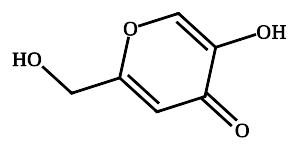
\includegraphics[width=3.2cm,height=0.9cm,keepaspectratio]{image/estruturas_ligantes_integracao/miniaturas/com_Acido_Kojico.png} & Estrutura química consultada no PubChem \parencite{pubchem2023} \\
Apigenina & 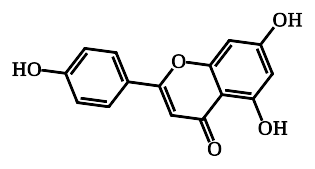
\includegraphics[width=3.2cm,height=0.9cm,keepaspectratio]{image/estruturas_ligantes_integracao/miniaturas/com_Apigenina.png} & Estrutura química consultada no PubChem \parencite{pubchem2023} \\
Arbutina & 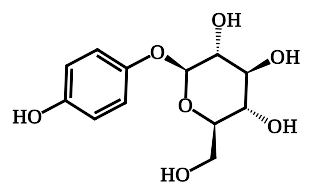
\includegraphics[width=3.2cm,height=0.9cm,keepaspectratio]{image/estruturas_ligantes_integracao/miniaturas/com_Arbutina.png} & Estrutura química consultada no PubChem \parencite{pubchem2023} \\
Batimastat & 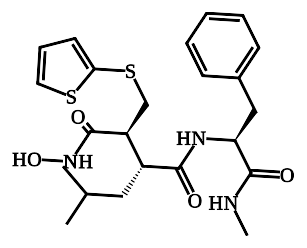
\includegraphics[width=3.2cm,height=0.9cm,keepaspectratio]{image/estruturas_ligantes_integracao/miniaturas/com_Batimastat.png} & Estrutura química consultada no PubChem \parencite{pubchem2023} \\
Cromoglicato & 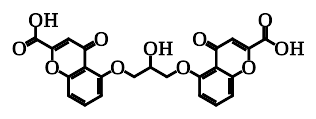
\includegraphics[width=3.2cm,height=0.9cm,keepaspectratio]{image/estruturas_ligantes_integracao/miniaturas/com_Cromoglicato.png} & Estrutura química consultada no PubChem \parencite{pubchem2023} \\
Doxiciclina & 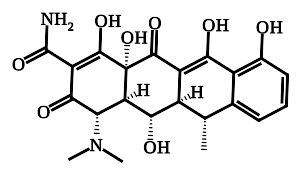
\includegraphics[width=3.2cm,height=0.9cm,keepaspectratio]{image/estruturas_ligantes_integracao/miniaturas/com_Doxiciclina.png} & Estrutura química consultada no PubChem \parencite{pubchem2023} \\
GW475151 & 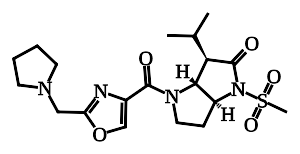
\includegraphics[width=3.2cm,height=0.9cm,keepaspectratio]{image/estruturas_ligantes_integracao/miniaturas/com_GW475151.png} & Complexo cristalográfico de elastase \parencite{macdonald2002} \\
Hidroquinona & 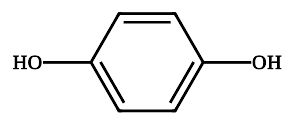
\includegraphics[width=3.2cm,height=0.9cm,keepaspectratio]{image/estruturas_ligantes_integracao/miniaturas/com_Hidroquinona.png} & Estrutura química consultada no PubChem \parencite{pubchem2023} \\
L2U & 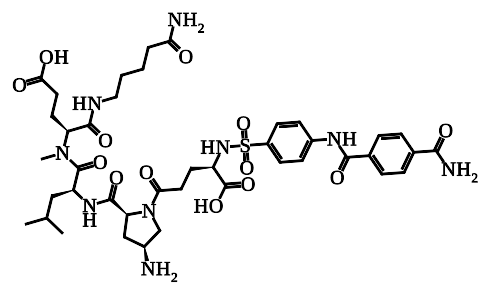
\includegraphics[width=3.2cm,height=0.9cm,keepaspectratio]{image/estruturas_ligantes_integracao/miniaturas/com_L2U.png} & Complexo cristalográfico de MMP-2 \parencite{takeuchi2023} \\
Marimastat & 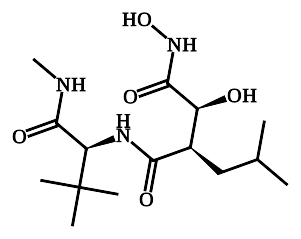
\includegraphics[width=3.2cm,height=0.9cm,keepaspectratio]{image/estruturas_ligantes_integracao/miniaturas/com_Marimastat.png} & Estrutura química consultada no PubChem \parencite{pubchem2023} \\
NFH & 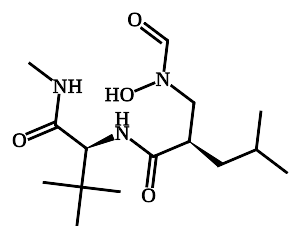
\includegraphics[width=3.2cm,height=0.9cm,keepaspectratio]{image/estruturas_ligantes_integracao/miniaturas/com_NFH.png} & Complexo cristalográfico de MMP-9 \parencite{rowsell2002} \\
PLH & 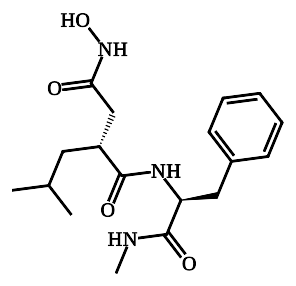
\includegraphics[width=3.2cm,height=0.9cm,keepaspectratio]{image/estruturas_ligantes_integracao/miniaturas/com_PLH.png} & Complexo cristalográfico de MMP-1 \parencite{spurlino1994} \\
Quercetina & 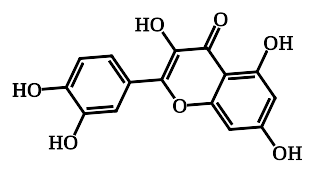
\includegraphics[width=3.2cm,height=0.9cm,keepaspectratio]{image/estruturas_ligantes_integracao/miniaturas/com_Quercetina.png} & Estrutura química consultada no PubChem \parencite{pubchem2023} \\
Sivelestat & 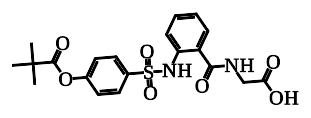
\includegraphics[width=3.2cm,height=0.9cm,keepaspectratio]{image/estruturas_ligantes_integracao/miniaturas/com_Sivelestat.png} & Estrutura química consultada no PubChem \parencite{pubchem2023} \\
Tropolona & 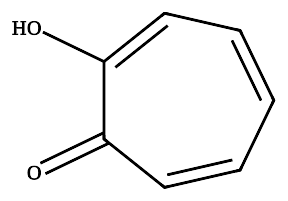
\includegraphics[width=3.2cm,height=0.9cm,keepaspectratio]{image/estruturas_ligantes_integracao/miniaturas/com_Tropolona.png} & Estrutura química consultada no PubChem \parencite{pubchem2023} \\
\end{longtable}
\normalsize
\renewcommand{\arraystretch}{1.25}
\setlength{\tabcolsep}{6pt}


\setlength{\LTpre}{0pt}
\setlength{\LTpost}{0pt}
\small
\renewcommand{\arraystretch}{1.1}
\setlength{\tabcolsep}{3pt}
\begin{longtable}{C{3.4cm}C{3.7cm}C{7.0cm}}
\caption{Compostos selecionados para prospecção, com desenhos do Apêndice B e fontes de ocorrência ou comparação.}\label{tab:ligantes_spe_justificativa}\\
\toprule Ligante & Estrutura bidimensional & Fonte da estrutura ou referência \\
\midrule
\endfirsthead
\multicolumn{3}{c}{\tablename~\thetable\ (continuação)}\\
\toprule Ligante & Estrutura bidimensional & Fonte da estrutura ou referência \\
\midrule
\endhead
\midrule
\multicolumn{3}{r}{Continua na próxima página}\\
\endfoot
\bottomrule
\endlastfoot
Ácido ferúlico & 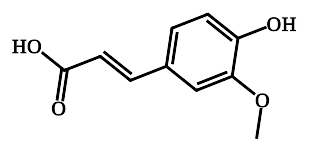
\includegraphics[width=3.2cm,height=0.9cm,keepaspectratio]{image/estruturas_ligantes_integracao/miniaturas/spe_Acido_Ferulico.png} & Extrato de biomassa de \textit{T. tetrahele} \parencite{mai2026} \\
Ácido galacturônico & 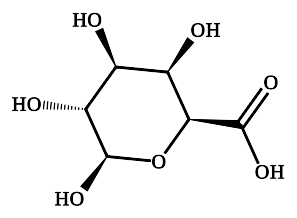
\includegraphics[width=3.2cm,height=0.9cm,keepaspectratio]{image/estruturas_ligantes_integracao/miniaturas/spe_Acido_Galacturonico.png} & Exopolissacarídeos de \textit{T. suecica} \parencite{parra2020} \\
Ácido gálico & 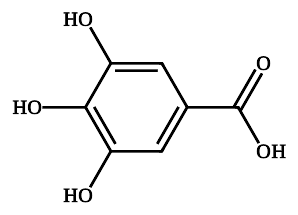
\includegraphics[width=3.2cm,height=0.9cm,keepaspectratio]{image/estruturas_ligantes_integracao/miniaturas/spe_Acido_Galico.png} & Extrato de biomassa de \textit{T. tetrahele} \parencite{mai2026} \\
Ácido glucurônico & 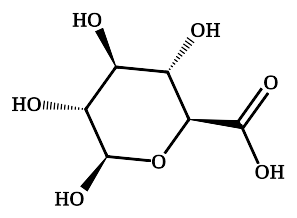
\includegraphics[width=3.2cm,height=0.9cm,keepaspectratio]{image/estruturas_ligantes_integracao/miniaturas/spe_Acido_Glucuronico.png} & Exopolissacarídeos de \textit{T. suecica} \parencite{parra2020} \\
D-Galactose & 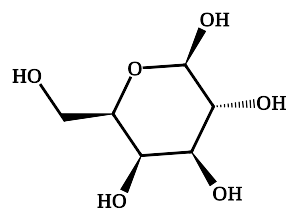
\includegraphics[width=3.2cm,height=0.9cm,keepaspectratio]{image/estruturas_ligantes_integracao/miniaturas/spe_D_Galactose.png} & Biomassa de \textit{T. chuii}; exopolissacarídeos de \textit{T. suecica} \parencite{brown1991,pereira2019,parra2020} \\
D-Glicose & 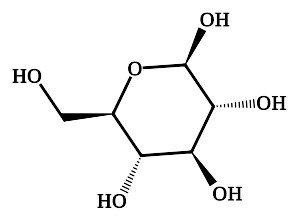
\includegraphics[width=3.2cm,height=0.9cm,keepaspectratio]{image/estruturas_ligantes_integracao/miniaturas/spe_D_Glicose.png} & Biomassa de \textit{T. chuii}; exopolissacarídeos de \textit{T. suecica} \parencite{brown1991,pereira2019,parra2020} \\
D-Gulose & 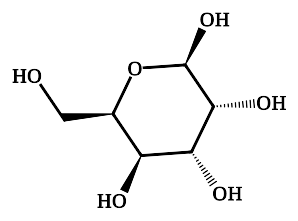
\includegraphics[width=3.2cm,height=0.9cm,keepaspectratio]{image/estruturas_ligantes_integracao/miniaturas/spe_D_Gulose_Raro_presente_na_SPE.png} & Parede celular de \textit{T. striata} \parencite{becker1989} \\
D-Manose & 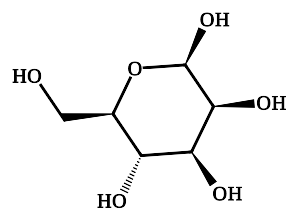
\includegraphics[width=3.2cm,height=0.9cm,keepaspectratio]{image/estruturas_ligantes_integracao/miniaturas/spe_D_Manose.png} & Biomassa de \textit{T. chuii}; exopolissacarídeos de \textit{T. suecica} \parencite{brown1991,pereira2019,parra2020} \\
D-Xilose & 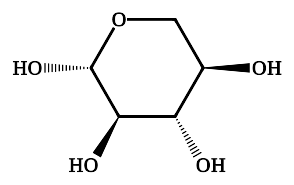
\includegraphics[width=3.2cm,height=0.9cm,keepaspectratio]{image/estruturas_ligantes_integracao/miniaturas/spe_D_Xilose.png} & Exopolissacarídeos de \textit{T. suecica} \parencite{parra2020} \\
\textit{Dha} & 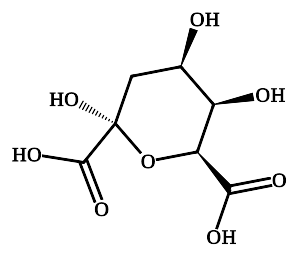
\includegraphics[width=3.2cm,height=0.9cm,keepaspectratio]{image/estruturas_ligantes_integracao/miniaturas/spe_Dha_3_deoxy_D_lyxo_hept_2_ulopyranosaric_acid.png} & Parede celular de \textit{T. striata} \parencite{becker1989} \\
Galactose-6-sulfato & 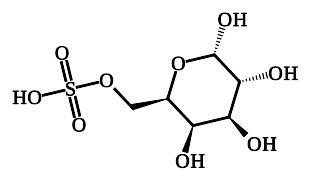
\includegraphics[width=3.2cm,height=0.9cm,keepaspectratio]{image/estruturas_ligantes_integracao/miniaturas/spe_Galactose_6_sulfato.png} & Comparador estrutural; sem fonte de ocorrência identificada \\
Glicose-6-sulfato & 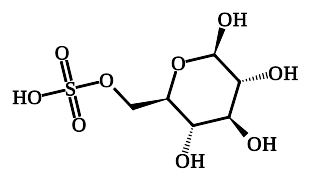
\includegraphics[width=3.2cm,height=0.9cm,keepaspectratio]{image/estruturas_ligantes_integracao/miniaturas/spe_Glicose_6_sulfato.png} & Unidades sulfatadas em polissacarídeos de \textit{Porphyridium} sp. \parencite{geresh2009} \\
KDO & 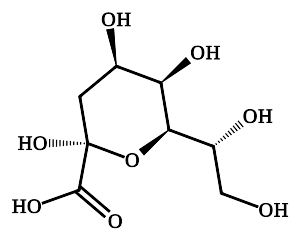
\includegraphics[width=3.2cm,height=0.9cm,keepaspectratio]{image/estruturas_ligantes_integracao/miniaturas/spe_KDO_3_deoxy_D_manno_oct_2_ulosonic_acid.png} & Parede celular de \textit{T. striata} \parencite{becker1989} \\
L-Arabinose & 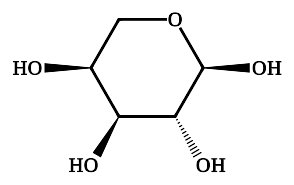
\includegraphics[width=3.2cm,height=0.9cm,keepaspectratio]{image/estruturas_ligantes_integracao/miniaturas/spe_L_Arabinose.png} & Biomassa de \textit{T. chuii}; exopolissacarídeos de \textit{T. suecica} \parencite{brown1991,pereira2019,parra2020} \\
L-Fucose & 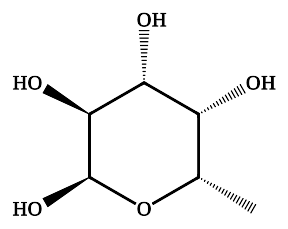
\includegraphics[width=3.2cm,height=0.9cm,keepaspectratio]{image/estruturas_ligantes_integracao/miniaturas/spe_L_Fucose.png} & Exopolissacarídeos de \textit{T. suecica} \parencite{parra2020} \\
L-Ramnose & 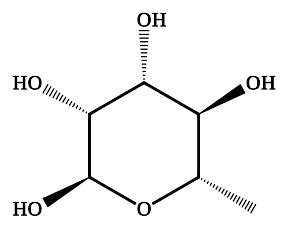
\includegraphics[width=3.2cm,height=0.9cm,keepaspectratio]{image/estruturas_ligantes_integracao/miniaturas/spe_L_Ramnose.png} & Biomassa de \textit{T. chuii}; exopolissacarídeos de \textit{T. suecica} \parencite{brown1991,pereira2019,parra2020} \\
$\alpha$-Kdo & 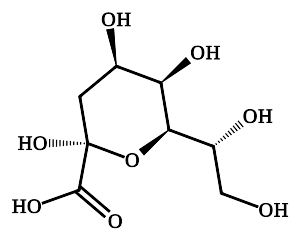
\includegraphics[width=3.2cm,height=0.9cm,keepaspectratio]{image/estruturas_ligantes_integracao/miniaturas/spe_alpha_Kdo_Isomero_comum_em_polissacarideos.png} & Comparador estrutural; sem fonte de ocorrência identificada \\
\end{longtable}
\normalsize
\renewcommand{\arraystretch}{1.25}
\setlength{\tabcolsep}{6pt}

